\chapter{Machine Learning Methods}\label{ch:3}
This chapter will treat the machine learning methods applied in this thesis. The subsection Support Vector Machines: \ref{Chapter:SVM}, will point out the idea of SVM including an introduction into the theoretical parts. Followed by: \ref{Chapter:PUL} where the Positive Unlabeled Learning (PUL) strategy for \textit{training} of our prediction model is discussed. The subjecting chapter: \ref{Chapter:OC-SVM} approach on One Class SVM, it will cover the concept and the gaps in respect to the ordinary SVM. At the end of this chapter, the subsection: \ref{Chapter:Ensemble} will introduce the concept of Ensembles in the scope of machine learning especially to improve the classification accuracy.

The purpose of the following introduction is:
\begin{itemize}
    \item Understand the core concept of the particular algorithms.
    
    \item Get a brief understanding of the theoretical concepts driving the algorithms.
    
    \item Became familiar with the possible tuning options that the algorithms contain and be able to track the motivation of adjusting them.
\end{itemize}
One last note before starting: the theoretical concepts will be presented in an aggregated form. The goal is to provide only the information necessary to follow up in the further chapter. 


\section[Support Vector Machines (SVM)] {Support Vector Machines (SVM) \footnote{The following chapter is based on the chapter 8 of the book~\cite{Okun;Valentini:2009}, and provides a brief summary of SVM important for further work in this thesis. } }\label{Chapter:SVM}

%http://stats.stackexchange.com/questions/63028/one-class-svm-vs-exemplar-svm
Support Vector Machines (SVM) \cite{Cortes;Vapnik:1995} is a well proven method with a solid background in statistical learning theory. It can be used for both classification and regression tasks. What distinguishes an SVM from other methods is a better ability to deal with high dimensional data and the guarantee of the globally optimal solution. The solution an SVM produces is sparse in many cases as only a fraction of training set instances is relevant for the task at hand. These instances, called support vectors, lie close to a hyperplane separating data into classes. Thus, an SVM tries to transform nonlinearly separable classes into linearly separable ones because the latter case is simpler to solve than the former. Without loss of generality and for the purpose of this thesis, only one or two classes are assumed to be present in the data.

Let us assume that we are given a data set as
\[  S = \{(x_1,y_2), (x_2,y_2), ...,(x_n,y_n) \} \; x_i \in \mathbf{R^d} \; y_i \in \{-1,1\}, \]
where \( x_i\) is the \( i-\)th input instance or data point and \( y_i\) is its class label. Thus, \(x_i\) is a \(d-\) dimensional column vector whereas \( y_i\) is a scalar.

A hyperplane that splits the data into two classes can be represented with the following equation:
\[\vec{w}^Tx + b = 0, \] 
where \(\vec{w}\) is a \textit{weight vector} determining the direction perpendicular to the hyperplane and \(b\) a \textit{bias} responsible for moving the hyperplane parallel to itself (see also\footnote{The figure is taken from the work of~\cite{Okun;Valentini:2009}}~\ref{fig:hyperplane1}).

\begin{figure}[h!]
    \centering % Picture from Oleg's book, do not forget the reffs!
    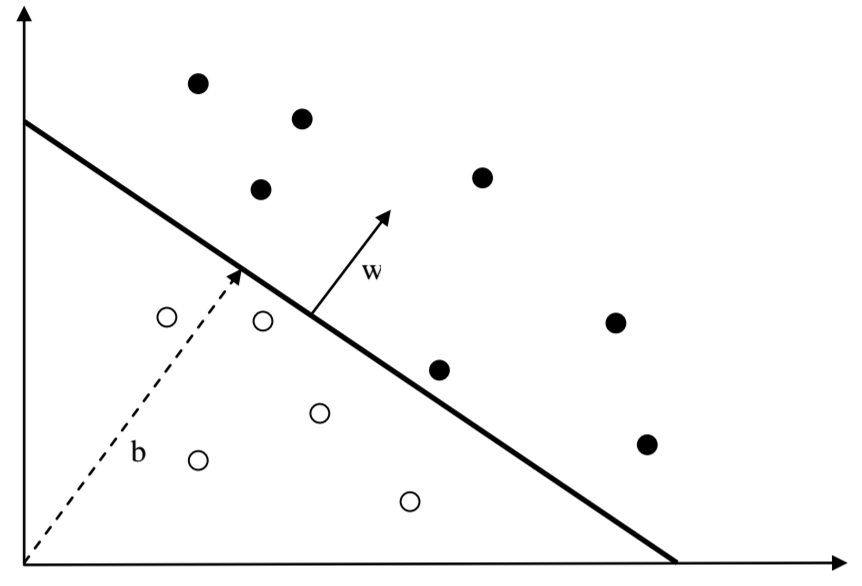
\includegraphics[scale=0.6]{Graphics/svm1.png}
    \caption{A hyperplane for separating 2-dimensional data.}
    \label{fig:hyperplane1}
\end{figure}

However, classes in the input space are often not linearly separable, which means that a linear classifier is not a good option in such a case. In the case of SVMs a solution is to project the original data into another, often a higher dimensional space \(x \mapsto \phi(x) \), where classes would more likely be linearly separable. Figure\footnote{The figure is taken from the work of~\cite{Okun;Valentini:2009}}~\ref{fig:hyperplane2} shows an example of input space \(X\) where data cannot be separated by a linear function. However after applying the mapping function \(\phi\) to each data point in \(X\), the data become well separable in a \textit{feature space} \(F = \{ \phi(x)\; | \; x \in X\}\).
\begin{figure}[h!]
    \centering
    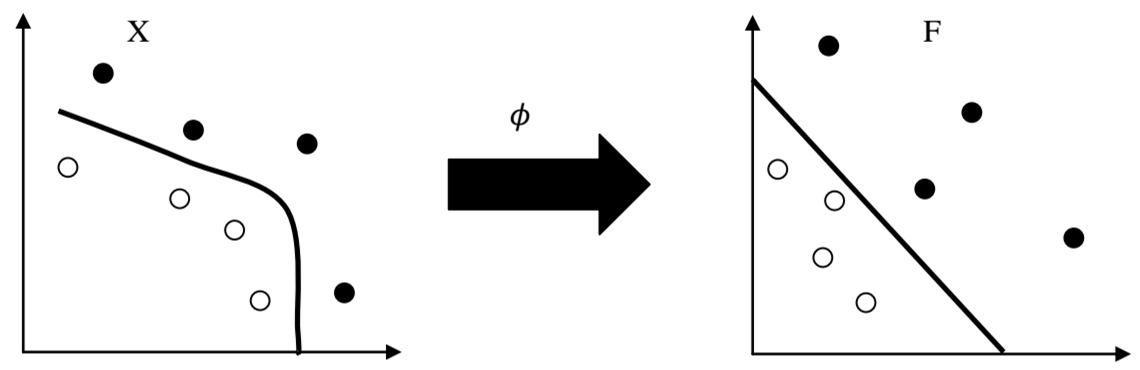
\includegraphics[scale=0.6]{Graphics/svp-separation.png}
    \caption{A visualization of mapping data into a feature space.}
    \label{fig:hyperplane2}
\end{figure}

Thus, a straightforward solution seems to transforms data into a feature space where a linear classifier can be built. These two operations are combined with the help of a kernel function. The typical kernel functions are:
\begin{itemize}
            \item \(K(x,z) = x'z \) - linear kernel
            \item \(K(x,z) = (\tau + x'z)^p\) - polynomial kernel of degree p
            \item \(K(x,z) = exp(-\sigma||x-z||^2)\) - Gaussian or Radial Basis Function (RBF) kernel
\end{itemize}

In these definitions, only $x$ and $z$ are vectors while other symbols denote scalars.

As one can see, the kernel representation eliminates the necessity to map each input individually: the inputs never appear isolated but in the form of inner products between pairs of vectors. Because of this, we don't need to know the underlying feature map! Also, the dimensionality of the feature space does not affect the computation as the inner product is a number. As a result, the only information that is necessary is a \(n\times n\) kernel matrix.

Kernels provide one pillar of SVMs. The other is the optimization theory as the SVM solution is formulated as an optimization task, subject to certain constraints. The primal optimization problem where \( w \) and \( b \) are involved is difficult to solve due to inequality constraints. Instead, the dual problem based on  Lagrangian theory \footnote{Lagrangian theory is a basic mathematical tool for constrained optimization of differentiable functions, especially for nonlinear constrained optimization \cite{Li:2008}.} transforms the task into a quadratic program where the function to be optimized is quadratic while the constraints are all equalities rather than inequalities. The solution of such a problem is known to be unique and global. It is also sparse by implying that only a small fraction of the original data matters for class separation, which results in a very efficient classifier.

Below both primal and dual optimization problems are given. The maximal (or hard) margin problem assumes two classes are only linearly separable in the feature space. To remedy its deficiency, the soft margin problem is then presented that works with nonlinearly separable classes by introducing slack variables measuring non-separability (see below).

The margin is a quantity indicating how well two classes of data are linearly separable. Figure\footnote{The figure is taken from the work of~\cite{Okun;Valentini:2009}}~\ref{fig:hyperplane3} shows the maximal margin $\gamma$ for a set of 2D points. Thus, the margin is a half distance between two hyperplanes parallel the class-separating hyperplane when this separation is maximized.
\begin{figure}[h!]
    \centering
    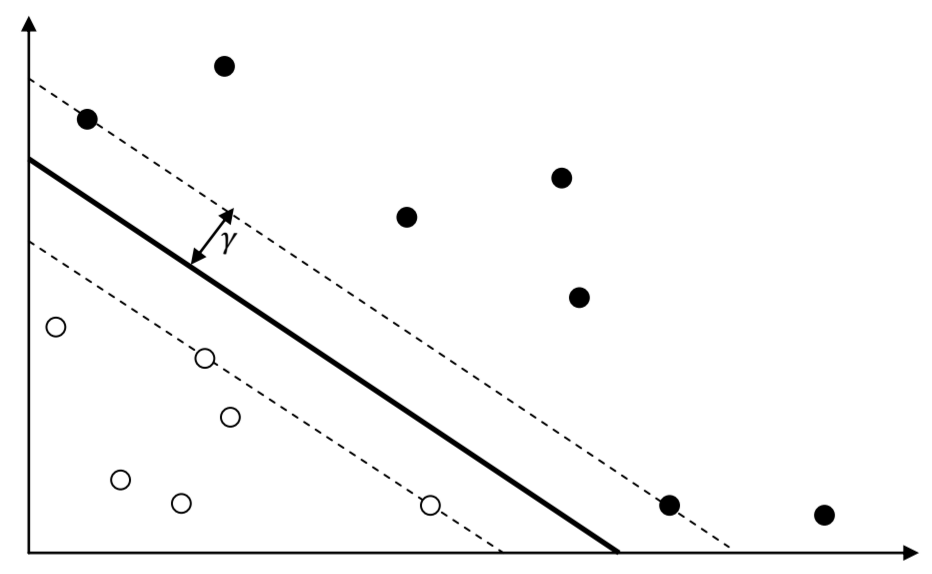
\includegraphics[scale=0.6]{Graphics/svm-margins.png}
    \caption{The margin of a set of points.}
    \label{fig:hyperplane3}
\end{figure}

\textbf{The maximal margin:}

\[\textrm{Primal problem:}\; \textrm{minimize}\; \vec{w} \vec{w},\] \[\textrm{subject to:}\; y_i(\vec{w}\vec{x_i} + b) \geq 1, i = 1, ...,l \] 

\[\textrm{Dual problem:}\; \textrm{maximize}\; W(a) =  \sum_{i=1}^{l} a_i - \frac{1}{2}\sum_{i,j = 1}^{l}a_i a_j y_i y_j K(\vec{x_i}^T \vec{x_j}), \] 
\[\textrm{subject to:}\; \sum_{i=1}^{l}a_i y_i = 0, a_i \geq 0, i = 1,...,l.\] 

\textbf{The 2-norm soft margin:}

\[\textrm{Primal problem:}\; \textrm{minimize}\; \vec{w} \vec{w} + C \sum_{i=1}^{l} \xi^2_i\; \textrm{over}\; \xi,\vec{w},b\] 
\[\textrm{subject to:}\; y_i(\vec{w}\vec{x_i} + b) \geq 1 - \xi_i,, i = 1, ...,l \] 

\[\textrm{Dual problem:}\; \textrm{maximize}\; W(a) =  \sum_{i=1}^{l} a_i - \frac{1}{2}\sum_{i,j = 1}^{l}a_i a_j y_i y_j \Big( K(\vec{x_i}^T \vec{x_j}) + \frac{1}{c}\delta_i \Big), \] 
\[\textrm{subject to:}\; \sum_{i=1}^{l}a_i y_i = 0, a_i \geq 0, i = 1,...,l.\] 

\textbf{The 1-norm soft margin:}

\[\textrm{Primal problem:}\; \textrm{minimize}\; \vec{w} \vec{w} + C \sum_{i=1}^{l} \xi_i\; \textrm{over}\; \xi,\vec{w},b\] 
\[\textrm{subject to}\; y_i(\vec{w}\vec{x_i} + b) \geq 1 - \xi_i,\xi_i \geq 0, i = 1, ...,l.\] 

\[\textrm{Dual problem:}\; \textrm{maximize}\; W(a) =  \sum_{i=1}^{l} a_i - \frac{1}{2}\sum_{i,j = 1}^{l}a_i a_j y_i y_j K(\vec{x_i}^T \vec{x_j}) , \]
\[\textrm{subject to}\; \sum_{i=1}^{l}a_i y_i = 0,C \geq a_i \geq 0, i = 1,...,l.\] 

\subsection{One Class SVM}\label{Chapter:OC-SVM}
\textit{One Class SVM} is an SVM-based classifier method proposed for cases when only one class of data is available to a modeler. Another important distinction from the conventional SVM is that instead of the separating hyperplane a hypersphere with minimal volume (or
minimal radius) containing all objects is sought \cite{Tax:2004:SVD:960091.960109}. 

As can be seen in the figure: \ref{fig:hypersphere} \footnote{The figure is takenn from the work of  \cite{s120810109}}, everything inside the sphere describes instances of a given class where outside lie outliers. 

\begin{figure}[h!]
    \centering
    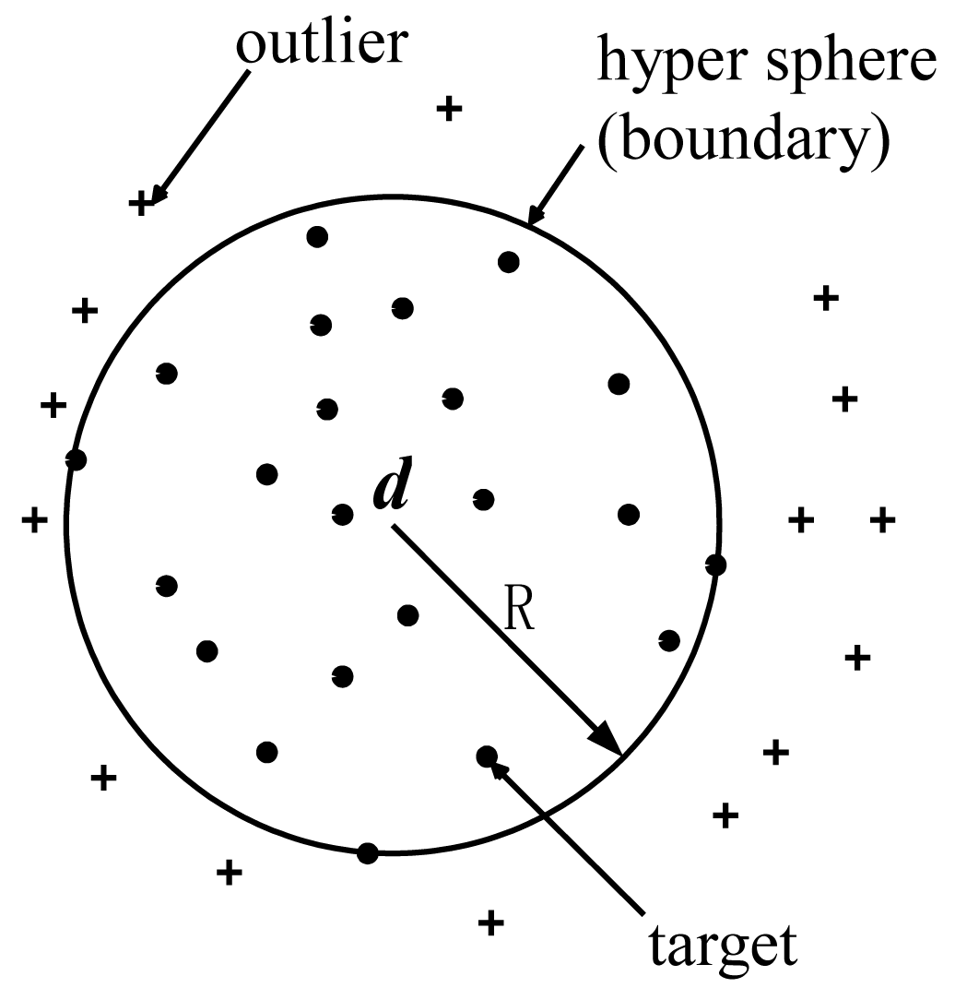
\includegraphics[scale=0.2]{Graphics/tax-duin-svm.png}
    \caption{A visualization of the classification with one-class SVM.}
    \label{fig:hypersphere}
\end{figure}

The resulting hypersphere is described by center \(d\) and radius
\(R\). Bellow the optimization problem is given: 

\[ \textrm{Minimize } R^2 + C \sum_{i=1}^{n} \xi_i, \]
\[ \textrm{subject to: } || x_i - d ||^2 \leq R^2 + \xi_i, \textrm{ } \xi_i \geq 0, \textrm{ } i = 1, ..., n \]

Where \( \xi \) are the slack variables for soft margin optimization and \( C \)  is the penalty parameter that gives the trade-off between the volume of the sphere and the number of errors.

\section[Positive and Unlabeled Learning]{Positive and Unlabeled Learning\footnote{The description and formulas of the Positive and Unlabeled Learning algorithm in this chapter are based on the work of \cite{Elkan;Noto:2008}.}}\label{Chapter:PUL}

Positive Unlabeled Learning (PUL) is an approach on the \textit{learning a classifier from positive and unlabeled data} problem. Because only one class is available (positive), PUL could be considered as a kind of one-class task. However, using unlabeled data, which are plenty, given modern data collection technologies, turns this task into two-class classification. Unlabeled data are assumed to contain both positive and negative instances but their labels are unknown to an observer. Because in PUL settings the amount of one class of data often far exceeds the amount of the other class, the classification problem becomes imbalanced. One of the ways to solve class imbalance is to use cost-sensitive learning where errors made on different classes have different costs.

The goal of the PUL technique by \cite{Elkan;Noto:2008} is to learn the true function \(f(.)\) that can predict the positive \(P\) examples as closely as possible, by learning another function \(g(.)\) from positive and unlabeled \(U\) data. Also a validation set, separate from the training data, is needed in order to find a normalizing constant \(c\) for \(g(.)\). After that, given a test (unseen) vector \(x\), \(f(x)\) is found as \(g(x)/c\).

PUL pseudocode is given below: \ref{alg:PUL}. 

\begin{algorithm}[h!]                      
\caption{PUL by using SVM.} 
\label{alg:PUL}                          
    \begin{algorithmic}[1]
        \State $ D\gets P \cup U$ \Comment{Positive and Unlabeled data, where Unlabeled is implicitly a label.}
        \State $\{Train,Valid,Test\}\gets split(D)$ \Comment{Split the original data into training, validation, and test sets.}
        \State $g \gets svm(Train)$ \Comment{Train a cost-sensitive 2-class SVM.}
        \State $Prob = g(Valid)$ \Comment{Get probabilities of being positive for positive instances of the validation set.}
        \State $c = mean(Prob)$ \Comment{Calculate the normalizing constant as the mean probability.} 
        \State $Prob = g(Test) / c$ \Comment{Compute the probability of being positive for test data.}
        \State If this probability is larger than 0.5, label a test instance as positive
   \end{algorithmic}
\end{algorithm}

There the data is first divided into training, validation, and test sets. Then a cost-sensitive SVM is used to train a classifier, able to predict the probability of an instance being positive. The result of applying the classifier on the validation set yields the normalizing constant (by taking the mean probability) that is then used for generating test set predictions.

In other works on PUL, experimental results showed that this approach significantly reduces the effort of labeling the data, while yielding competitive results, compared to the case when both positive and negative labels must be known before learning (see \cite{Li:2011}).

\section{PUL Ensemble}\label{Chapter:Ensemble}
\textit{PUL Ensemble} is an approach to combine multiple PUL algorithms in order to improve classification performance and outperform a single PUL algorithm. One of the common techniques to create an ensemble is to associate a separate training set with each ensemble member. In this thesis we selected the Robust Ensemble of Support Vector Machines algorithm \cite{Claesen:2014} in order to implement the ensemble.

The problem of PU learning can be considered as a supervised task with label noise in the negative set \cite{Claesen:2014}. However, the assumption that only the negative set can contain label noise can be violated due to various reasons \cite{journals/tnn/FrenayV14}. For example, our assumption that borrowers which have already paid at least one installment back are believed not having fraudulent intentions (see Chapter ~\ref{Ch:2:Overview}) could be violated when some borrowers are paying a small amount of money back in order to hide their fraudulent intentions - that would mean those positive examples \(P\) can contain label noise.

Robust Ensemble of Support Vector Machines (RESVM) is an ensemble algorithm with the goal to improve classification performance of PU Learning tasks where label noise is assumed to be present in both positive and negative sets of instances \cite{Claesen:2014}. The RESVM is based on following two methods that already treat the problem of label noise in \(U\):

\textit{Bagging SVM} algorithm by ~\cite{journals/prl/MordeletV14}, which consists of aggregating SVM trained on random resamples of \(U\) to discriminate \(P\). 

\textit{Class-weighted SVM (CWSVM)} is a classification technique where the penality parameter for misclassifications \(C\) differs from class to class \cite{conf/icdm/LiuDLLY03}. Applied to a PU Learning problem the misclassification of positive examples is penalized more than the misclassification of unlabeled examples to emphasize the higher degree of certainty on positive labels \cite{Claesen:2014}.

Additionally to that, the RESVM introduces the concept of resampling both \(P\) and \(U\), compared to the Bagging SVM where only \(U\) is resampled. Resampled sets will have a different amount of label noise without increasing the bias. Training based on randomly resampled sets decreases the variance and thus increases the classification accuracy \cite{journals/ml/Breiman00}.

As our implementation of the PUL algorithm is also based on class weighted penalties, CWSVM is in fact identical to a single PUL algorithm.

Below the algorithm of RESVM is given \ref{alg:RESVM}.

\begin{algorithm}[h!]                      
\caption{RESVM} 
\label{alg:RESVM}
\begin{algorithmic}[0]
        \State $ n_{models}  $ \Comment{Number of base models (SVM) in the ensemble.}
         \State $ n_{unl}  $ \Comment{Size of resample of \(U\) .}
        \State $ n_{pos}  $  \Comment{Size of resample of \(P\) .}
        \State $ k(.)  $  \Comment{Kernel function to be used by SVM.}
        
\end{algorithmic}
    \begin{algorithmic}[1]
       \State $\Omega    \gets \emptyset$  \Comment{Output with \(n_{models}\) base models.}
        % \State $ C_p \gets C_U \times w_{pos} \times \frac{n_{unl}}{n_{pos}} $  \Comment{Kernel function to be used by SVM.}
        \For{i:=1}{ $n_{models}$ }
            \State $P^i \gets sample(P,n_{pos}) $ \Comment{Sample \(n_{pos}\) instances with replacement from \(P\).}
            \State $U^i \gets sample(U,n_{unl}) $ \Comment{Sample \(n_{unl}\) instances with replacement from \(U\).}
            \State $ D^i \gets  P^i \cup U^i$ \Comment{Combine two sets of instances to form a training set.}
            \State $\psi^i \gets train(D^i,k) $ \Comment{Train CWSVM to discriminate \(P\) vs \(U\), with kernel \(k\).}
            \State $\Omega \gets \Omega \cup \psi^i $ \Comment{Add a trained model to the output.}
        \EndFor{\textbf{end for}}
   \end{algorithmic}
\end{algorithm}

In each iteration, a random sample of \(P\) and \(U\) is drawn (with replacement) separately. Then both samples are combined to form a training set for a Class-Weighted SVM (\(P\) vs \(U\)). Once all ensemble members have been trained, the final prediction is defined by a majority voting. In case of a tie, a random decision is made.


